%gibt an: Papierformat, einseitiger Druck, Schriftgr��e
\documentclass[a4paper,oneside,titlepage,12pt]{article}
%-------------------------------------------------------------------
\usepackage[a4paper, top=2cm, footskip=0pt, headheight=0.8cm, headsep=0.6cm, lmargin=3cm, rmargin=2cm]{geometry}
\usepackage{graphicx}
\usepackage{helvet}
\usepackage{amsmath}
\usepackage{amsthm}
\usepackage{amssymb}
\usepackage{hyperref} 
\usepackage[right]{eurosym}
\usepackage[latin1]{inputenc}

%--------------------------------------------------------------------
\renewcommand{\baselinestretch}{1.2}

\begin{document}
%--------------------------------------------------------------------
%Titelseite
\begin{titlepage}
	
\includegraphics{grafiken/HTW-Logo.png}
	%
\includegraphics[width=.3\textwidth]{grafiken/HTW-Logo.png}
	\vspace*{3cm}
	\begin{center}
		\Huge{Android-Zusammenfassung\\} \vspace*{1cm}
		\huge{Felix Krautschuk\\}
		\small{(Matrikelnummer: 34230)}
		\vspace*{2cm}
		\normalsize{
			\\Studiengang Informatik\\
		}
	\end{center}
	\vspace{2cm}
\begin{center}
\large{ 5. Semester }
\end{center}
	\vspace*{3cm}



\end{titlepage}

\thispagestyle{empty}\clearpage

%----------------------------------------------------------------------------------------------------------------
%\rmfamily \pagestyle{fancy} \setcounter{secnumdepth}{4}
\newtheorem{satz}{Satz}
\newtheorem{lemma}[satz]{Lemma}
\newtheorem{folgerung}[satz]{Folgerung}
\theoremstyle{definition}
\newtheorem{definition}[satz]{Definition}
\numberwithin{equation}{section}
\renewcommand{\proofname}{Beweis}

\pagenumbering{roman}\setcounter{page}{3} \tableofcontents
\newcounter{roemisch} \setcounter{roemisch}{\value{page}}
\clearpage

\setcounter{page}{2} \pagenumbering{arabic}
%-----------------------------------------------------------------------------------------------------------------

\section{Programmstruktur - die wichtigsten Verzeichnisse und Dateien}
\includegraphics{grafiken/ordnerstruktur.jpg}

\subsection{AndroidManifest.xml}
Zu jeder App geh�rt eine zentrale Beschreibungsdatei. Sie enth�lt eine Liste der
Komponenten, aus denen das Programm besteht und befindet sich in der obersten
Ebene des Projektverzeichnisses. Au�erdem werden in ihr die ben�tigten
Berechtigungen sowie etwaige zus�tzlich verwendete Bibliotheken vermerkt. Auch
Angaben zur mindestens n�tigen oder gew�nschten Android-Version werden hier
eingetragen.
\\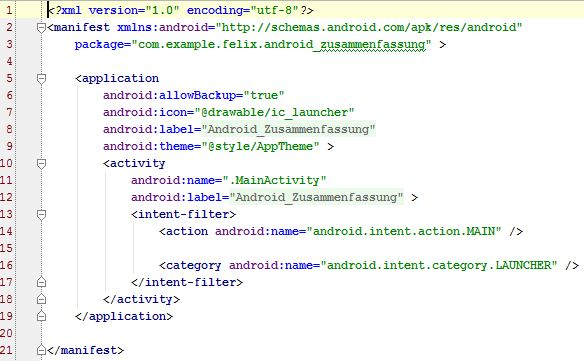
\includegraphics{grafiken/leereAppAndroidManifest}
\\Die Komponenten einer Anwendung sind Kinder des Elements
\textit{\textless application/\textgreater}. Wenn man im Assistenten zum Anlegen
neuer Projekte Create Activity mit einem H�kchen versieht und einen Namen
eintr�gt, enth�lt das Manifest ein Element \textit{\textless activity
/\textgreater}. Dessen Attribut android:name beinhaltet den im Assistenten
eingegebenen Activity-Namen. Wenn man manuell eine Activity-Klasse anlegt (eine
Klasse anlegt und mit \textit{extends Activity} versieht), muss man nachtr�glich
die erzeugte Activity im Manifest bekannt machen. Mithilfe des Elementes
\textit{\textless intent-filter /\textgreater} kann man eine Activity zur
Haupt-Activity machen. Dessen Kindelement \textit{\textless action
/\textgreater} kennzeichnet die Activity als Haupteinstiegspunkt in die
Anwendung. \textit{\textless category /\textgreater} sorgt daf�r, dass sie im
Programmstarter angezeigt wird.

\subsection{strings.xml}
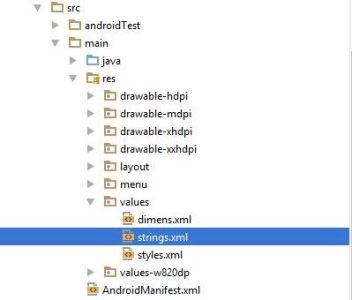
\includegraphics{grafiken/leereAppStrings.jpg}
\\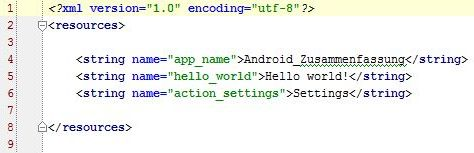
\includegraphics{grafiken/leereAppStrings1.jpg}
\\Elemente haben einen Titel. �blicherweise werden s�mtliche Titel in die
String-Resource Datei \textit{string.xml} eingetragen und �ber
\textit{@string/\ldots} referenziert. Die Speicherung von Texten an einem
zentralen Ort hat zahlreiche Vorteile. Beispielsweise werden identische
Textteile leichter entdeckt, als wenn diese in den Quelltexten der Klassen
verborgen sind und man erst jede Klasse oder Layout-Datei durchsuchen muss.
Damit l�sst sich, wenn auch in eher bescheidenem Umfang, Speicherplatz sparen.
Au�erdem macht die Trennung von Daten und Programmlogik die
Internationalisierung, also die �bersetzung einer App in verschiedene Sprachen,
viel einfacher. Hierzu wird f�r jede zu unterst�tzende Sprache im Ordner
\textit{res} ein Verzeichnis angelegt.
Dessen Name beginnt mit \textit{values-} und endet mit dem ISO-Sprachschl�ssel.
F�r Deutsch ist dies \textit{de}. Das Verzeichnis muss also \textit{values-de}
hei�en. Jeder dieser Ordner erh�lt eine eigene Version von \textit{strings.xml}.
Deren Bezeichner sind stets gleich, die Texte liegen hingegen in den jeweiligen
Sprachen vor. Texte in der Standardsprache verbleiben in \textit{values}.

\subsection{main.xml}
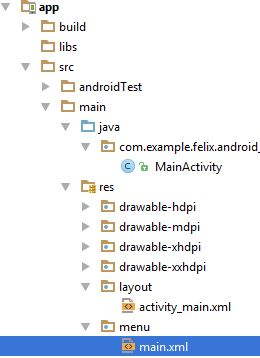
\includegraphics{grafiken/leereAppMenue2.jpg}
\\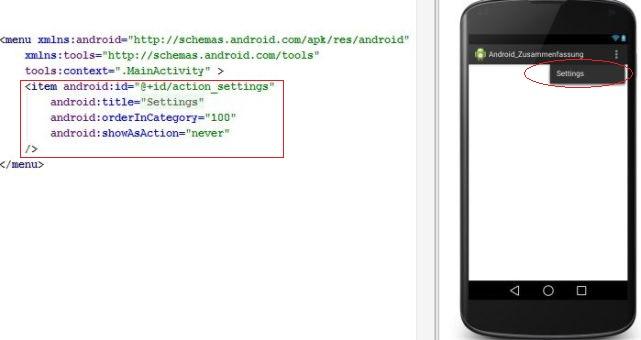
\includegraphics{grafiken/leereAppMenue.jpg}
\\Die \textit{main.xml} ist eine sogenannte Menu-Resource-Datei.
Menu-Resource-Dateien sind im Verzeichnis '\textit{src/menu}' hinterlegt und
dienen dazu Options-Men�s oder Kontextmen�s zu erstellen (Erl�uterungen dazu im
sp�teren Kapitel Men�s), die man z.B. mit der Men�taste des Smartphones
bet�tigen aufrufen kann. Men�-Items sollten immer in solchen Men�-Dateien
aufgebaut werden statt in den Activity-Dateien. Man kann die erstellten Men�s
sp�ter in Activities oder Fragments einbinden.
\subsection{activity\_main.xml}
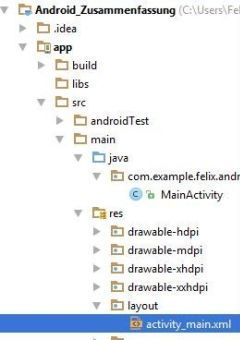
\includegraphics{grafiken/leereActivityLayout.jpg}
\\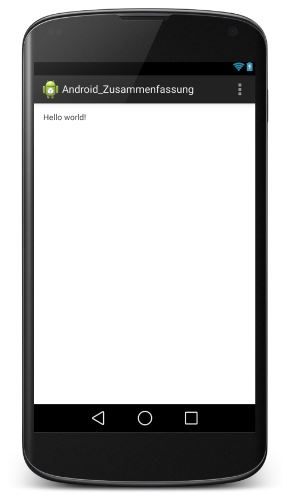
\includegraphics{grafiken/leereActivityLayout2.jpg}

\section{Layouts, Views und Komponenten}
\subsection{Layouts}
\subsection{Views und Widgets}
%S.117 Android 4 Apps mit SDK
\subsection{Basiskomponenten einer App}
\subsubsection{Activity}
Normalerweise ist jeder Activity eine Benutzeroberfl�che, also ein Baum bestehend
aus Views und ViewGroups, zugeordnet. Activities bilden demnach die vom Anwender
wahrgenommenen Bausteine einer App.
Sie repr�sentieren also meist die Benutzeroberfl�che und Interaktionen. 
Jede Android- Anwendung besteht deshalb aus mindestens einer Activity.
Activities k�nnen andere Activities aufrufen und mit ihnen Daten austauschen.
Jede Activity besteht aus einer in XML definierten Layout-Datei und einer
dazugeh�rigen Java-Klassendatei, welche bei Android Studio im Verzeichnis
\\'\textit{\%Appname/src/main/java/\%packagename/}' abgelegt ist. Die
dazugeh�rige Layout-Datei (XML-Datei) ist im Verzeichnis
'\textit{\%Appname/src/main/res/layout}' zu finden.

%S.95 Android 4 Apps mit SDK
%onCreate()
%onCreateOptionsmenu
%onOptionsItemSelected(MenuItem item)


\subsubsection{Intents}
%S. 102 Android 4 Apps mit SDK
%S. 82  Android Apps mit Beispiel realer App
%Implizite und Explizite Intents
\subsubsection{Fragments}
%S. 109 Android 4 Apps mit SDK
\subsubsection{Services}
\subsubsection{Men�s}
%Kontextmen�s, Optionsmen�s
%http://developer.android.com/guide/topics/ui/menus.html
%http://developer.android.com/guide/topics/resources/menu-resource.html
%S.85 Android Apps mit Beispiel realer App

\section{Allgemeiner Ablauf bei einer einfachen Beispiel-App}
\subsection{Anlegen eines Projektes und Erstellung einer MainActivity}

\subsection{Layout festlegen und Views hinzuf�gen}
\subsection{ID und Namen eines jeden Views festlegen}
%string.xml!
\subsection{Einbinden der View-Elemente in die Activity-Klasse}
%findViewById(R.id. ..)
\subsection{Actionbar mit Image-Buttons erstellen}
%S. 76 Android Apps entwickeln Beispiel realer App
\subsection{Intents zum Aufruf einer Activity aus der aktuellen Activity}
\subsection{Anmelden der Activities im Manifest}


\end{document}
